%%%%%%%%%%%%%%%%%%%%%%%%%%%%%%%%%%%%%%%%%%%%%%%%%%%%%%%%%%%%%%%%%%%%%%%%%%%%%%%%
% Template for USENIX papers.
%
% History:
%
% - TEMPLATE for Usenix papers, specifically to meet requirements of
%   USENIX '05. originally a template for producing IEEE-format
%   articles using LaTeX. written by Matthew Ward, CS Department,
%   Worcester Polytechnic Institute. adapted by David Beazley for his
%   excellent SWIG paper in Proceedings, Tcl 96. turned into a
%   smartass generic template by De Clarke, with thanks to both the
%   above pioneers. Use at your own risk. Complaints to /dev/null.
%   Make it two column with no page numbering, default is 10 point.
%
% - Munged by Fred Douglis <douglis@research.att.com> 10/97 to
%   separate the .sty file from the LaTeX source template, so that
%   people can more easily include the .sty file into an existing
%   document. Also changed to more closely follow the style guidelines
%   as represented by the Word sample file.
%
% - Note that since 2010, USENIX does not require endnotes. If you
%   want foot of page notes, don't include the endnotes package in the
%   usepackage command, below.
% - This version uses the latex2e styles, not the very ancient 2.09
%   stuff.
%
% - Updated July 2018: Text block size changed from 6.5" to 7"
%
% - Updated Dec 2018 for ATC'19:
%
%   * Revised text to pass HotCRP's auto-formatting check, with
%     hotcrp.settings.submission_form.body_font_size=10pt, and
%     hotcrp.settings.submission_form.line_height=12pt
%
%   * Switched from \endnote-s to \footnote-s to match Usenix's policy.
%
%   * \section* => \begin{abstract} ... \end{abstract}
%
%   * Make template self-contained in terms of bibtex entires, to allow
%     this file to be compiled. (And changing refs style to 'plain'.)
%
%   * Make template self-contained in terms of figures, to
%     allow this file to be compiled. 
%
%   * Added packages for hyperref, embedding fonts, and improving
%     appearance.
%   
%   * Removed outdated text.
%
%%%%%%%%%%%%%%%%%%%%%%%%%%%%%%%%%%%%%%%%%%%%%%%%%%%%%%%%%%%%%%%%%%%%%%%%%%%%%%%%

\documentclass[lettersize,journal]{IEEEtran}
% \usepackage{usenix2019_v3}

% to be able to draw some self-contained figs
\usepackage{tikz}
\usepackage{amsmath}

% inlined bib file
\usepackage{filecontents}
\usepackage{cite}
\usepackage{amsmath,amssymb,amsfonts}
% \usepackage{algorithmic}
\usepackage{graphicx}
\usepackage{textcomp}
\usepackage{tabularx}
\usepackage{subcaption}
\usepackage{makecell}
\usepackage{url}
\usepackage[switch]{lineno}
% \linenumbers
\usepackage{listings}
\usepackage{multirow}
% \usepackage[xcdraw]{xcolor}
% \usepackage{graphicx}
% \usepackage{textcomp}
% \usepackage{tabularx}
% \usepackage{adjustbox}

\captionsetup{compatibility=false}
\usepackage[margin=0.5in]{geometry}
\usepackage{textcomp}

% \usepackage{bera}% optional: just to have a nice mono-spaced font
\usepackage{listings}
% \usepackage{xcolor}

\colorlet{punct}{red!60!black}
\definecolor{background}{HTML}{EEEEEE}
\definecolor{delim}{RGB}{20,105,176}
\colorlet{numb}{magenta!60!black}

% %-------------------------------------------------------------------------------
% \begin{filecontents}{\jobname.bib}
% %-------------------------------------------------------------------------------
% @Book{arpachiDusseau18:osbook,
%   author =       {Arpaci-Dusseau, Remzi H. and Arpaci-Dusseau Andrea C.},
%   title =        {Operating Systems: Three Easy Pieces},
%   publisher =    {Arpaci-Dusseau Books, LLC},
%   year =         2015,
%   edition =      {1.00},
%   note =         {\url{http://pages.cs.wisc.edu/~remzi/OSTEP/}}
% }
% @InProceedings{waldspurger02,
%   author =       {Waldspurger, Carl A.},
%   title =        {Memory resource management in {VMware ESX} server},
%   booktitle =    {USENIX Symposium on Operating System Design and
%                   Implementation (OSDI)},
%   year =         2002,
%   pages =        {181--194},
%   note =         {\url{https://www.usenix.org/legacy/event/osdi02/tech/waldspurger/waldspurger.pdf}}}
% \end{filecontents}


\begin{document}

\title{ Sentiment Analysis on Hotel Reviews}

\author{Siva Teja Segu , Pavansai Pottimuthi, Ajith Reddy Busipally, Sreehari Revuri\\

Kent State University}
        % <-this % stops a space
% \thanks{This paper was produced by the IEEE Publication Technology Group. They are in Piscataway, NJ.}% <-this % stops a space
% \thanks{Manuscript received April 19, 2021; revised August 16, 2021.}}

 %The paper headers
%\markboth{Journal of \LaTeX\ Class Files,~Vol.~14, No.~8, August~2021}%
%{Shell \MakeLowercase{\textit{et al.}}: A Sample Article Using IEEEtran.cls for IEEE Journals}

% \IEEEpubid{0000--0000/00\$00.00~\copyright~2021 IEEE}
% Remember, if you use this you must call \IEEEpubidadjcol in the second
% column for its text to clear the IEEEpubid mark.

\maketitle

%-------------------------------------------------------------------------------
%\begin{abstract}
  %-------------------------------------------------------------------------------
  
%TODO: Write your abstract here

  
%\end{abstract}

%\begin{IEEEkeywords}
 % NLP, BOW (Bag of words), Stemming and lemmatization, TF-IDF (Term Frequency and Inverse Dense Frequency), Word2vec, Random Forest Classifier, ROC and AUC: Precision and Recall
  %\end{IEEEkeywords}

%\maketitle


%-------------------------------------------------------------------------------
\section{Introduction}
%-------------------------------------------------------------------------------
Sentiment analysis plays a key role in the field of Natural Language Processing, and it is a technique that extract emotions from the raw texts. Most of the E-Commerce sites like Amazon, Flipkart and Google etc., has wide range of applications built on this. Say, for example think about google translator application. It performs brilliantly in understanding, analyzing and translating the data. Also, it is effectively used on social media post and customer reviews in order to know the opinion of the customers whether they are happy or not with product, service and other factors which will play key role in enhancing their businesses. 
\subsection{Background}
Sentiment analysis, commonly referred to as opinion mining, is a process that uses machine learning, statistical methods, and natural language processing to recognize and extract subjective information from textual data, such as views, attitudes, and emotions. To ascertain the general attitude or sentiment that is being represented in a text is the main objective of sentiment analysis.

A hotel review is a written assessment of a guest's stay at a hotel that is often published on an internet platform such as a travel website or social media. Hotel evaluations may include details about a guest's experience with the rooms, staff, and facilities, as well as their overall happiness with their stay.
\subsection{ Problem Statement}
The objective of the project to perform sentimental analysis on a hotel review dataset. Given a review by its customers, we need to predict whether the review is good or bad review in other words say it is positive or negative.
For each textual review, we want to predict if it corresponds to a good review (the customer is happy) or to a bad one (the customer is not satisfied).
\subsection{Why is it important}
As it enables organizations to analyse massive volumes of unstructured data effectively and economically, sentiment analysis is proven to be a useful tool. As a way to divide reviews, it is becoming more and more popular. It is easy to use and can be occasionally simply adjusted. It gives facts and quantifiable data for upcoming decision-making, and when done well, it delivers value to a business. Sentiment research should be used by businesses that want to improve their goods and services, increase sales, and outwit their rivals.

\subsection{Plans to implement}
To swiftly determine whether a review is good or negative, sentiment analysis is required. This paper offers a solution by utilizing the Random Forest Classifier, Word2Vec approach to categorize positive and negative opinion reviews, and by comparing models using preprocessing, feature extraction, and feature selection. Due to their communities' stronger inclination toward data science, such as NLP and Deep Learning for Sentiment Analysis, open-source libraries in programming languages like Python and Java are particularly well suited to creating specialized Sentiment Analysis solutions. But, this demanded a lot of time, money up front, and resources.

\section{Literature Review}
One of the main tools that a machine may use to comprehend human psychology is sentiment analysis. In order to be used in domains where people were previously required to identify mood or emotion, this technology is currently the subject of substantial research. It plays a key role in chat bot assistants, and when paired with speech recognition technology, it may also be used to replace people in contact centers. 

\par For NLP, machine learning methods were introduced. Several of the systems created during this time period employed machine learning methods such as decision trees to build systems of hard if-then rules comparable to existing hand-written rules. In NLP, the hidden Markov models employed part-of-speech tagging, and certain statistical models that make probabilistic judgments were developed. For sentiment categorization, there are five different machine learning classifiers: Nave Bayes, K-Nearest Neighbor, Support Vector Machine, Logistic Regression, and Random Forest.[1]

Nandal in this paper classified amazon product reviews for sentiment analysis using SVM(Support Vector Machine) Tool. The study examined how words can shift in meaning depending on the context in which they're used, and how this impacts the overall evaluation of a product and its specific features.[2].

 \par Humera Shaziya classified movie reviews for sentiment analysis using WEKA Tool. They enhanced the earlier work done in sentiment categorization which analyzes opinions which express either positive or negative sentiment
[3].

Ahmad Kamal designed an opinion mining framework that facilitates objectivity or subjectivity analysis, feature extraction and review summarizing.He used supervised machine learning approach for subjectivity and objectivity classification of reviews. The various techniques used by him were Naive Bayes, Decision Tree, Multi layer Perception and Bagging. He also improved mining performance by preventing irrelevant extraction and noise.[4].\par

Orestes Appel used natural language processing (NLP)essential techniques, a sentiment lexicon enhanced with the assistance of SentiWordNet,and fuzzy sets to estimate the semantic orientation polarity and its intensity for sentences,
which provides a foundation for computing with sentiments. The proposed hybrid method is applied to three different data-sets and the results achieved are compared to those obtained
using Naive Bayes and Maximum Entropy techniques[5].
\section{Proposed Model}
The research began with an examination of many research and review articles on sentiment analysis, and each publication's summary was prepared by reading and comprehending the document. Examine popular classification techniques such as Nave Bayes, Random Forest, k-nearest neighbor, Decision Tree Induction, and Support Vector Machine.

The information was obtained from Booking.com. This dataset includes 515,000 customer reviews and ratings for 1493 premium hotels throughout Europe. In the meanwhile, the geographical location of hotels is supplied for additional examination.

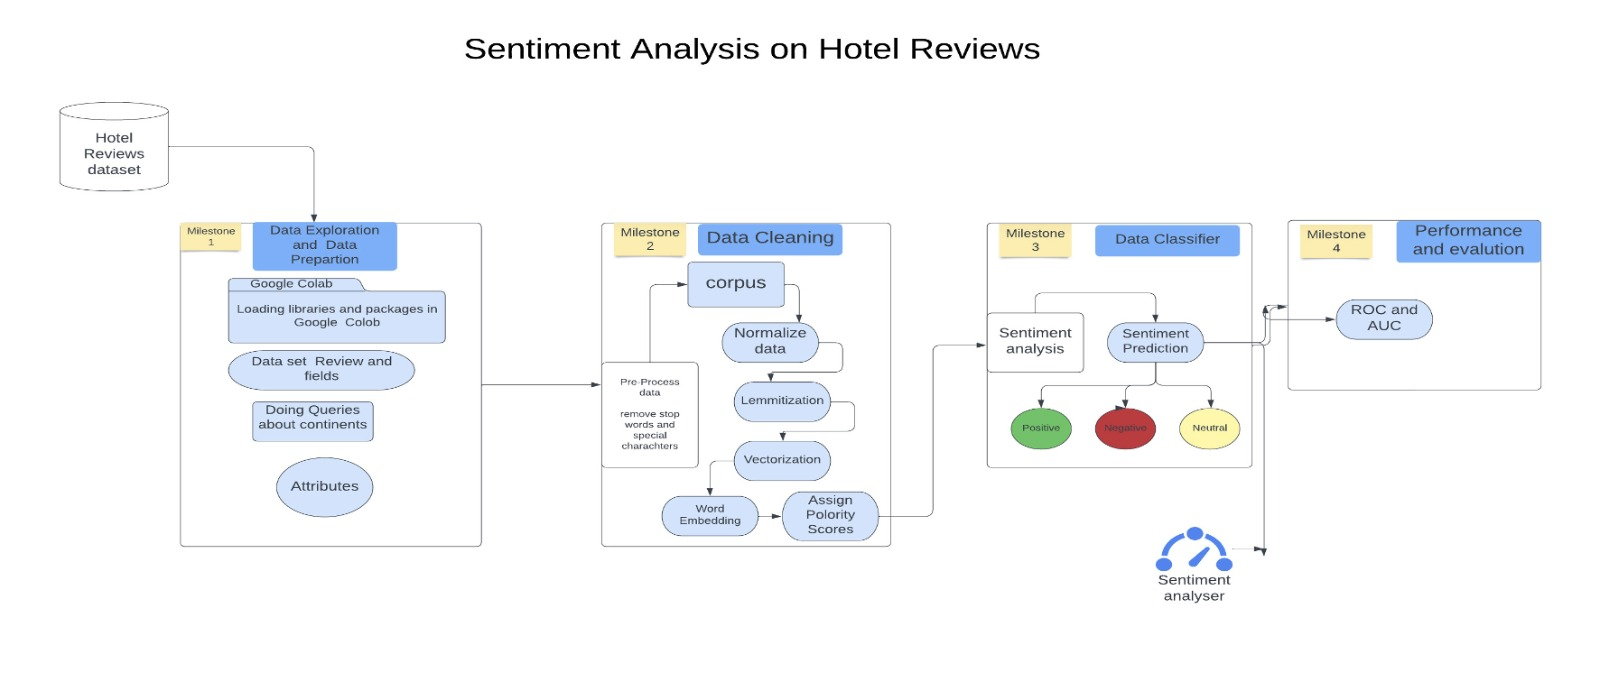
\includegraphics[width=9cm, height=6cm \textwidth]{block.jpeg}
\subsection{Data preparation and data exploration}

Pandas describe method will give some statistical parameters of the data set like count, mean and standard deviation.

\subsection{Data cleaning is the fundamental step in any NLP techniques}
\begin{itemize}

\item Data Cleaning and preprocessing steps.
\item Using gensim module to convert the text to vectors using DOC2VEC function 
\item By using SentimentIntensityAnalyzer we find the polarity scores and plot word cloud.
\end{itemize}

\subsection{ Classification}

We are using Random forest and Transformers Using RoBERTa

\subsection{Performance Evaluations }

A receiver operating characteristic (ROC) and area under the curve (AUC).
Precision Recall curve(PR) we are using for performance and evaluation.
\section{Key Concepts}
\subsection{Overview of Dataset}
As we have taken dataset from booking.com. The CSV file contains 17 fields. The description of each field is as below
\begin{itemize}
\item Hotel\_Address: Address of hotel.
\item Review\_Date: Date when reviewer posted the corresponding review.
\item Average\_Score: Average Score of the hotel, calculated based on the latest comment in the last year.
\item Hotel\_Name: Name of Hotel
\item Reviewer\_Nationality: Nationality of Reviewer
\item Negative\_Review: Negative Review the reviewer gave to the hotel. If the reviewer does not give the negative review, then it should be: 'No Negative'
\item ReviewTotalNegativeWordCounts: Total number of words in the negative review.
\item Positive\_Review: Positive Review the reviewer gave to the hotel. If the reviewer does not give the negative review, then it should be: 'No Positive'
\item ReviewTotalPositiveWordCounts: Total number of words in the positive review.
\item Reviewer\_Score: Score the reviewer has given to the hotel, based on his/her experience
\item TotalNumberofReviewsReviewerHasGiven: Number of Reviews the reviewers has given in the past.
\item TotalNumberof\_Reviews: Total number of valid reviews the hotel has.
\item Tags: Tags reviewer gave the hotel.
\item dayssincereview: Duration between the review date and scrape date.
\item AdditionalNumberof\_Scoring: There are also some guests who just made a scoring on the service rather than a review. This number indicates how many valid scores without review in there.
\item lat: Latitude of the hotel
\item lng: longitude of the hotel
\end{itemize}
\subsection{Data Cleaning}
In Data Cleaning we follow set of processes like Normalizing the data, Stemming and lemmatization, Word2Vec, Wordembeding, and Vectorization.

\section{ Libraries }
\subsection{NLTK}
The popular open-source library  Natural Language Toolkit (nltk) makes working with human language data in Python straightforward. It provides a wide range of NLP methods, including as sentiment analysis, part-of-speech tagging, tokenization, stemming, lemmatization, and named entity recognition, among others.
\subsection{SentimentIntensityAnalyzer}
It is a rule-based sentiment analyzer, and depending on their semantic orientation, sentences are frequently labeled as either positive or negative. Lastly, we use the polarity scores technique to determine the emotion.
\subsection{Gensim}
The gensim library is an open-source Python library for topic modeling and similarity detection in large and complex text datasets.The Gensim algorithms Word2Vec, FastText, Latent Semantic Indexing where it automatically recognize the semantic structure of documents by examining statistical  occurrences patterns within a corpus of training texts. There is no need for human input because these algorithms are unsupervised.
\subsection{Google Colab Software}
Google Colab is a free to use Jupyter notebook environment where we can create and run Python code in a web browser. By making GPU-accelerated computing resources and pre-installed machine learning libraries accessible, it is made to encourage collaborative work and study.It is an effective  tool for projects involving data science and machine learning, especially those that call for access to huge datasets and substantial processing capacity.
\section{ Infrastructure }
\subsection{GPU machine}
we are using GPU machines which are  available from a variety of cloud computing providers, such as Amazon Web Services, Microsoft Azure, and Google Cloud. By using GPU machine we can greatly accelerate the training and inference of machine learning models, reducing the time required to train and test models.It is expensive for long term project.
\section{Research Methods }
\subsection{Data Preparation and Data Exploration}
We have used Google Colob space for our project, in first step we have to give path of our dataset so that it will read and then we can do explotary data analysis. To get a quick overview of the data set we use the dataframe.info() function.Python is an excellent language for data analysis, due
to the solid ecosystem of data-centric Python tools.

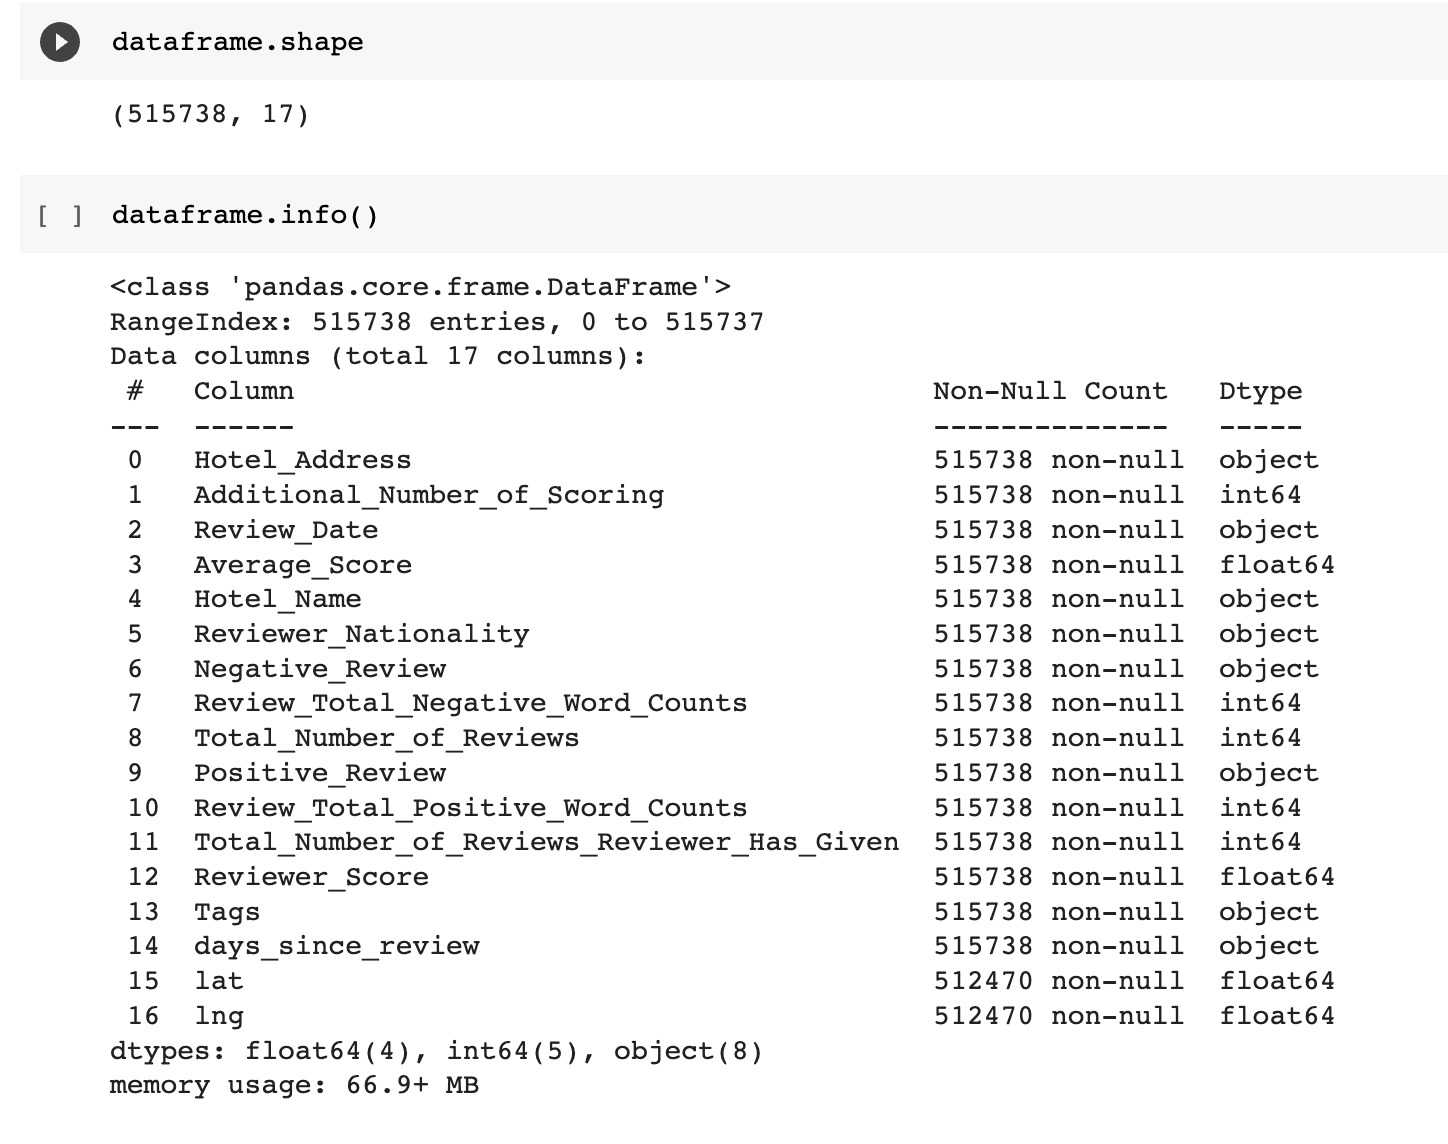
\includegraphics[width=9cm, height=6cm \textwidth]{dataframe.jpeg}
Pandas method will give us some of the statistical parameters
of the dataset like count, mean and standard deviation.
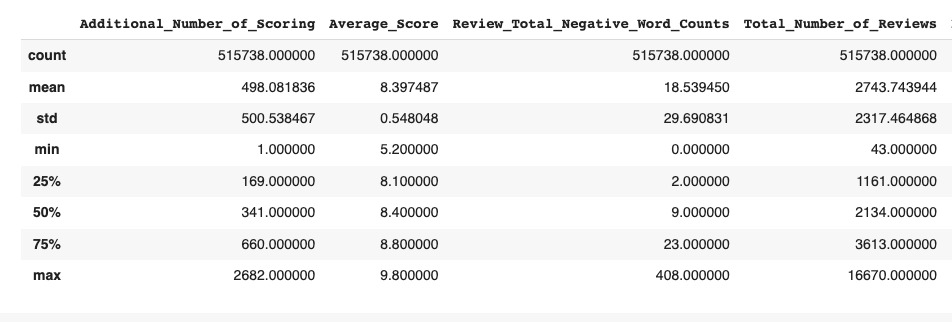
\includegraphics[width=9cm, height=6cm \textwidth]{f.jpeg}
After exploring the dataset there is only Reviewer nationality data in the dataset, so in order to find from which city, country and continent customers visited the hotels.Using countrycity dataset we added new coloumn to the dataset 'Hotel\_city\_country'.
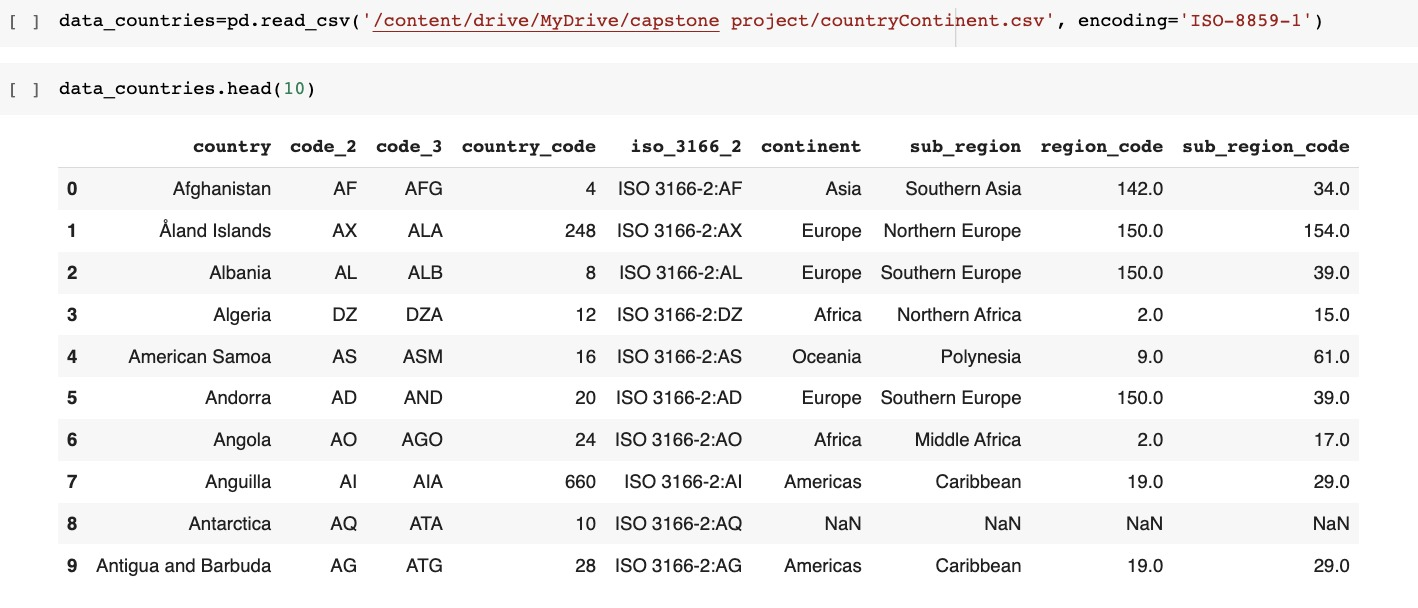
\includegraphics[width=10cm, height=10cm \textwidth]{country.jpeg}
In the below visualization we can see distribution hotel city country, customers visiting hotels are highest from United Kingdom and least is from Milan Italy.
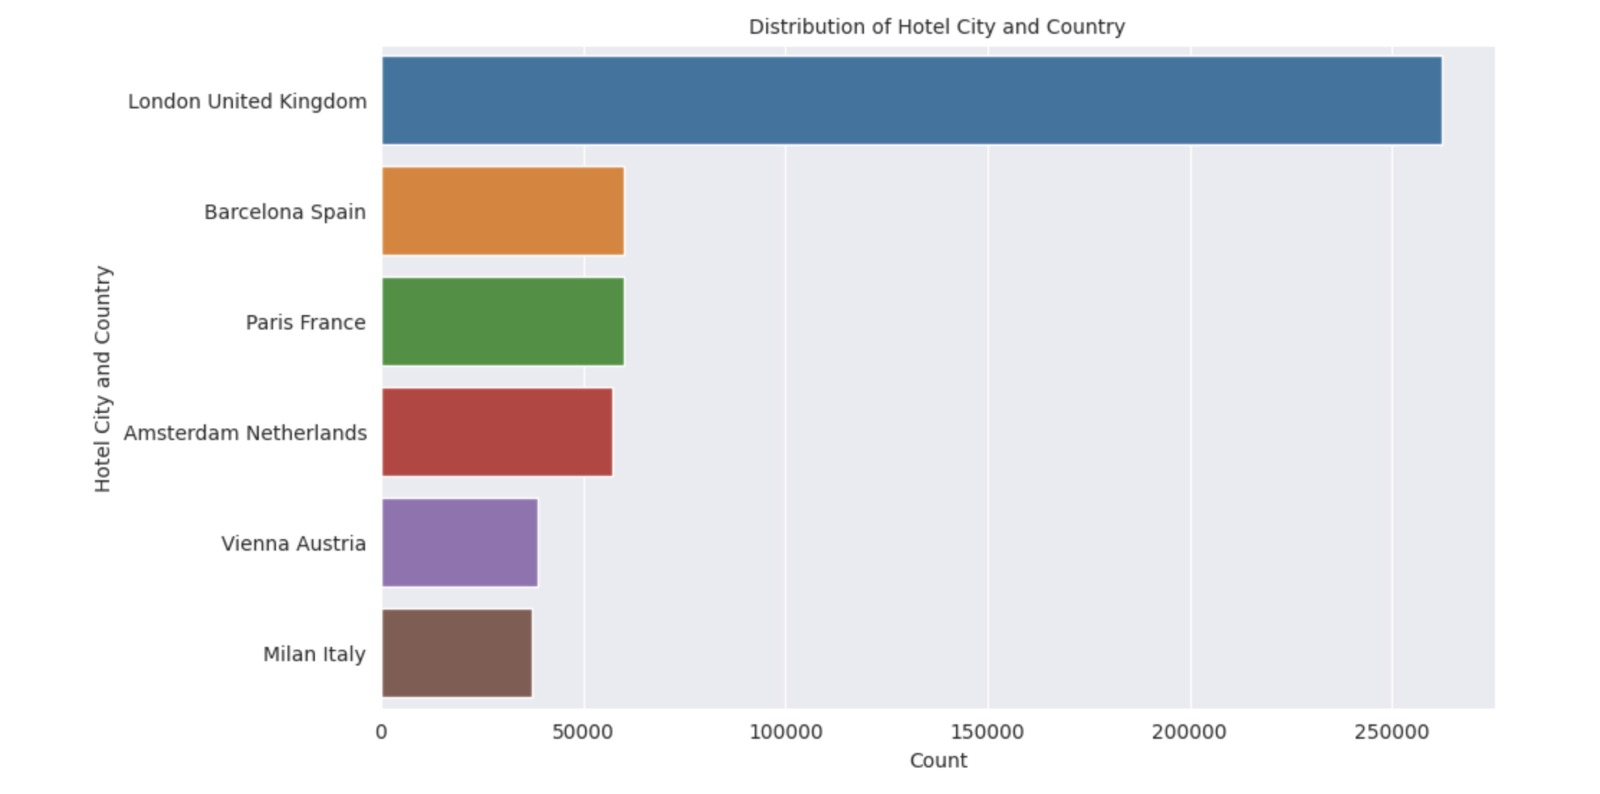
\includegraphics[width=9cm, height=9cm \textwidth]{hotelcitycountry.jpeg}

 In order to see if there is any outliers in the dataset we are using Boxplot will be useful one, after plotting there are outliers in our dataset in some of the coloumns there are outliers those should be cleaned or manipulated to bring under standard normal distribution.\\
 
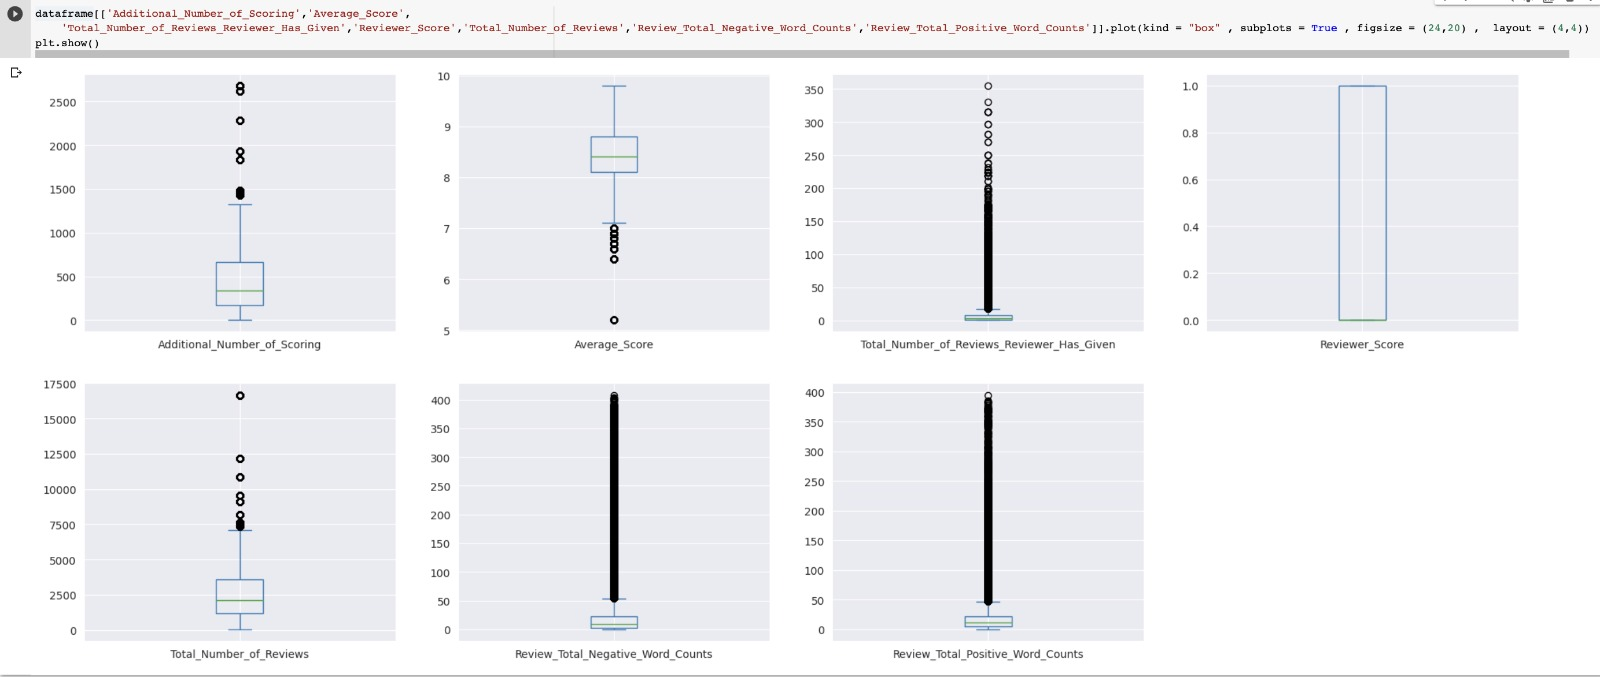
\includegraphics[width=9cm, height=6cm \textwidth]{Boxplot.jpeg}

To find correlation among other variables in the dataset we plotted correlation using heatmaps. The further away the correlation coefficient is from zero, the stronger the relationship between the two variables.\\

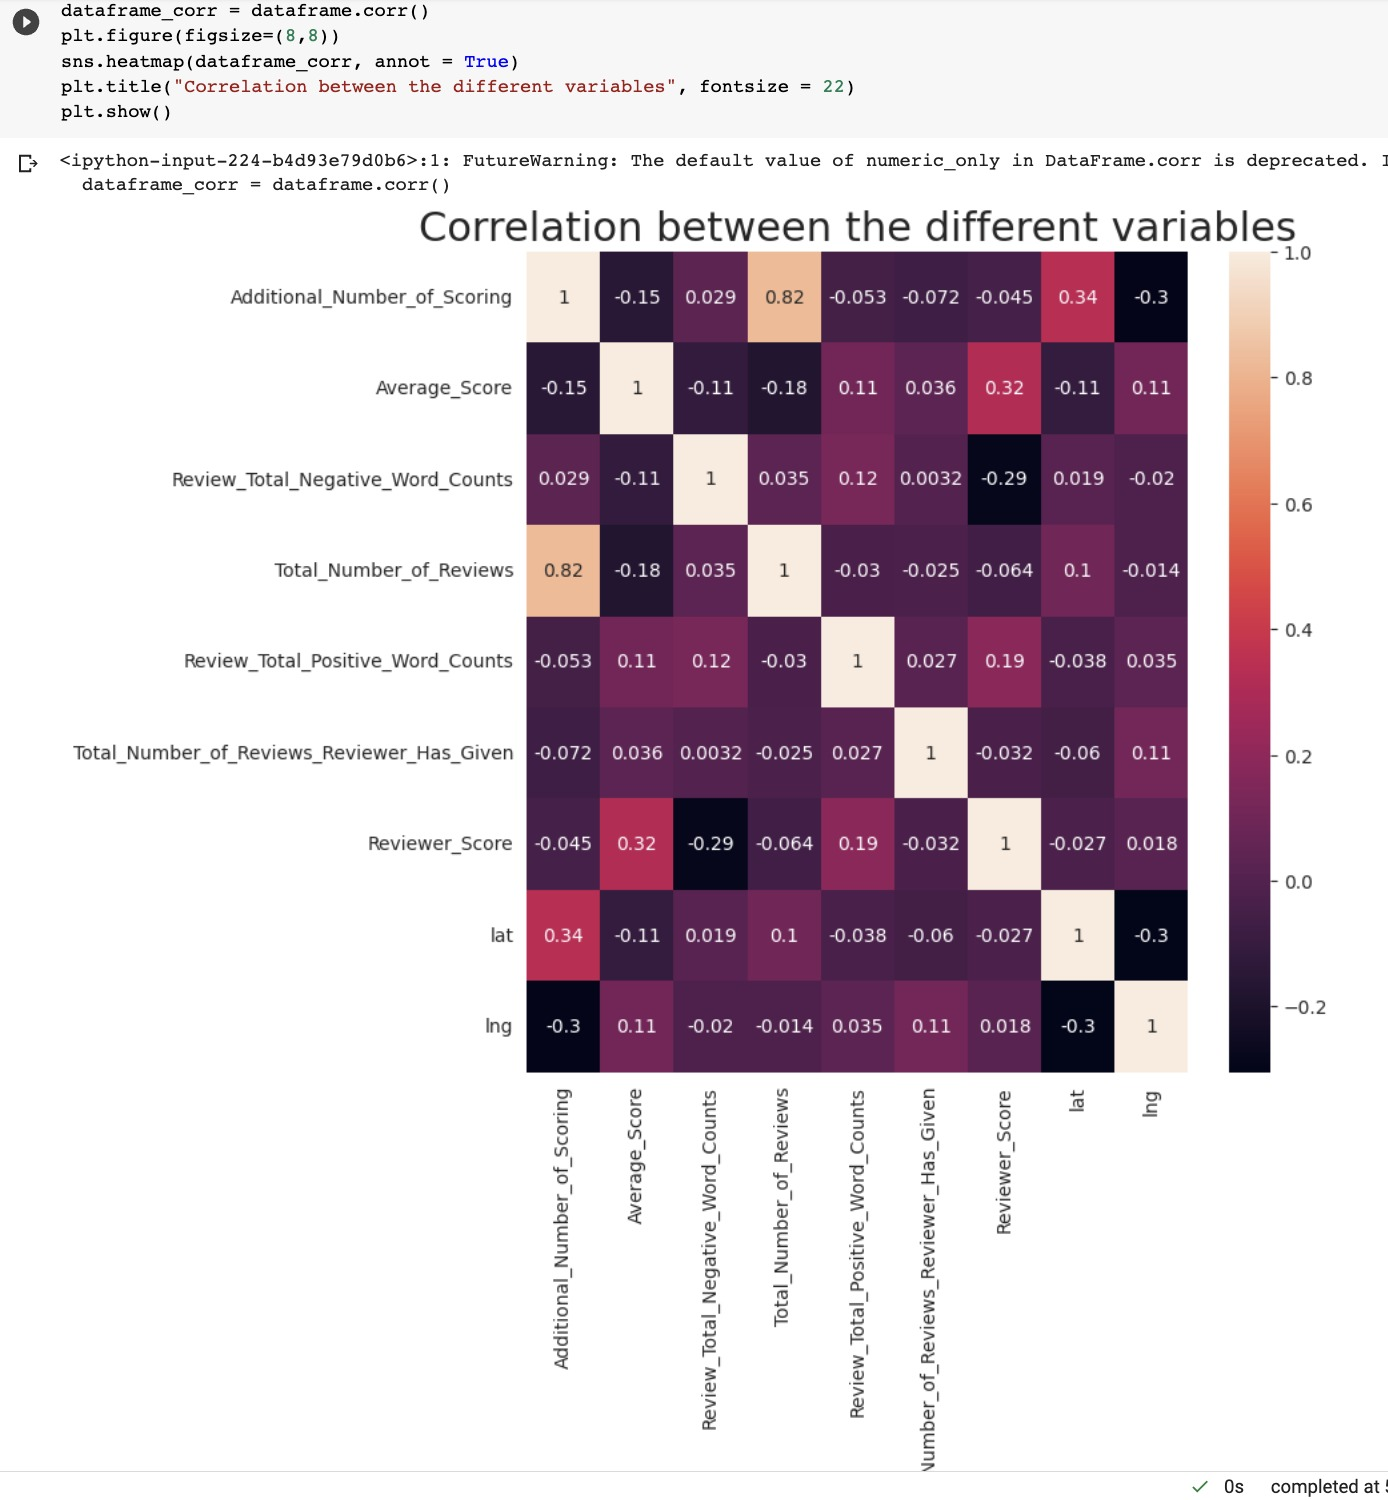
\includegraphics[width=9cm, height=9cm \textwidth]{ccorellation.jpeg}
\\
\subsection{Data Cleaning}
After exploring dataset the next step is Data Cleaning. In this step data is cleaned in many steps.Data cleaning is the fundamental step in any NLP techniques. The below code represents that we are doing the following processes
\begin{itemize}

\item Convert the sentences to lower case letter as a step for preprocessing.
\item Remove special symbols like “”, !,@,\#,\$ in our data.
\item Remove stop words and remove tokens like tags.
\item Tokenization, lemmatization.
\item Remove no negatives and no positives from data.
\item Clean textual data using parts of speech.

\end{itemize}
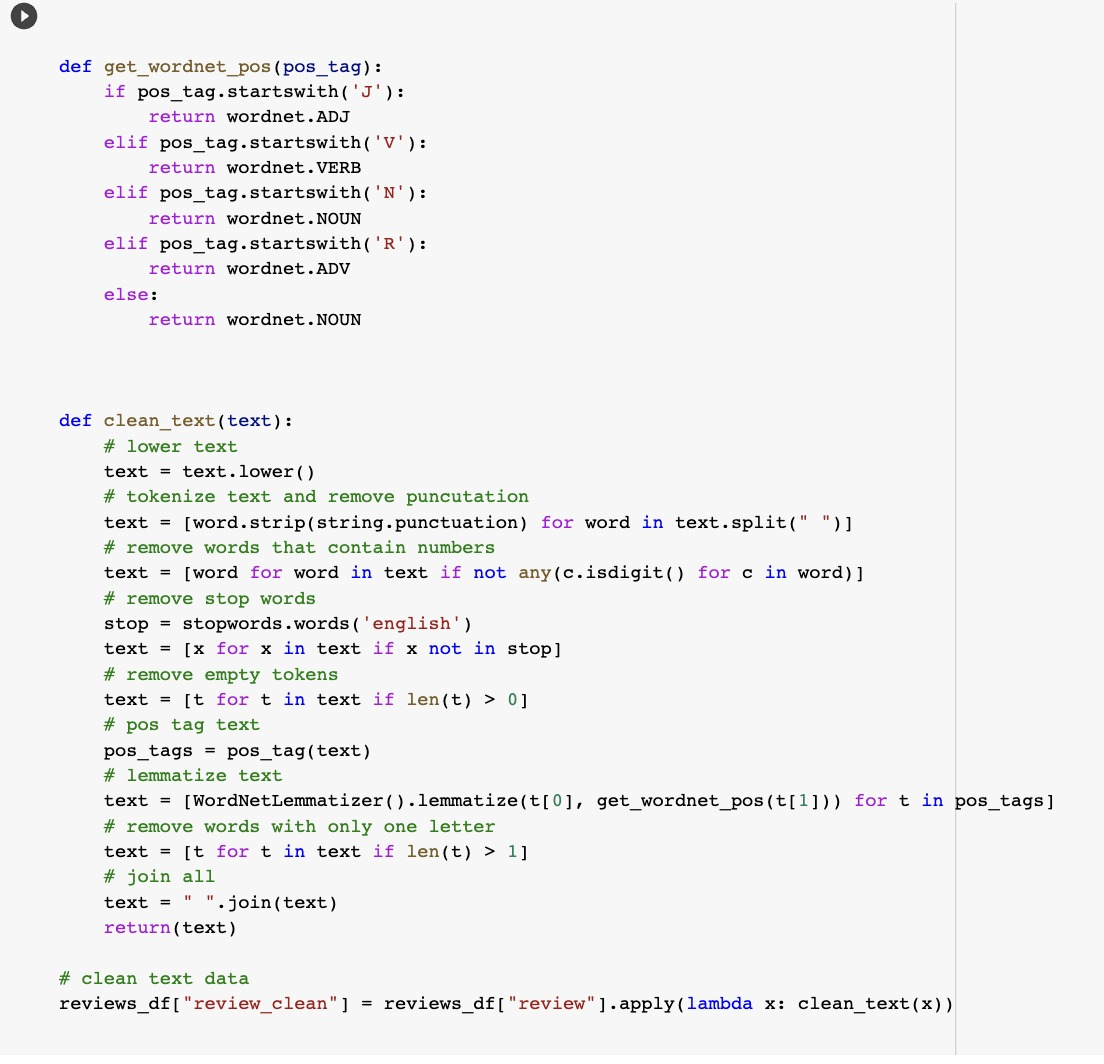
\includegraphics[width=9cm, height=9cm \textwidth]{data cleaning.jpeg}
\subsubsection{Bag Of Words (BOW)}
Raw text is initially reprocessed and after processing and cleaning techniques.
\subsubsection{Cleaned or preprocessed }
Remove all unnecessary special characters, if there are words of other accent like polish, German, Spanish etc. Remove or replace them or add the right Unicode to make them readable for machine. 
\subsubsection{Normalize all Data}
Make the data properly in a single case letter, either upper or lower. Preferred lower using .lower() function.
\subsubsection{Stemming and lemmatization}
In this methods used by search engines and chat bots to analyze the meaning behind a word. Stemming uses the stem of the word, while lemmatization uses the context in which the word is being used.

\subsubsection{Term Frequency and Inverse Dense Frequency(TF-IDF )}

Inverse document frequency looks at how common (or uncommon) a word is amongst the document.

IDF =Log [(\# Number of documents) / (Number of documents containing the word)]

Term frequency works by looking at the frequency of a particular term you are concerned with relative to the document.

	 TF = (Number of repetitions of word in a document) / (\# of words in document).
  
For combined TF – IDF = TF(t, d) * IDF(t)

So, using TF and IDF machine makes sense of important words in a document and important words throughout all documents.

\subsubsection{Word2vec}
It is a combination of models where it represents distributed of words in a corpus C. Here, it is an algorithm which accepts  input corpus and outputs as vector representation for each word.Word embeddings are numerical representations of words that capture their semantic meaning, used in various NLP tasks such as text classification, sentiment analysis, and machine translation.Word2Vec creates a dense vector representation for each word, allowing us to explore semantic relationships between words.
\subsubsection{SentimentIntensityAnalyzer}
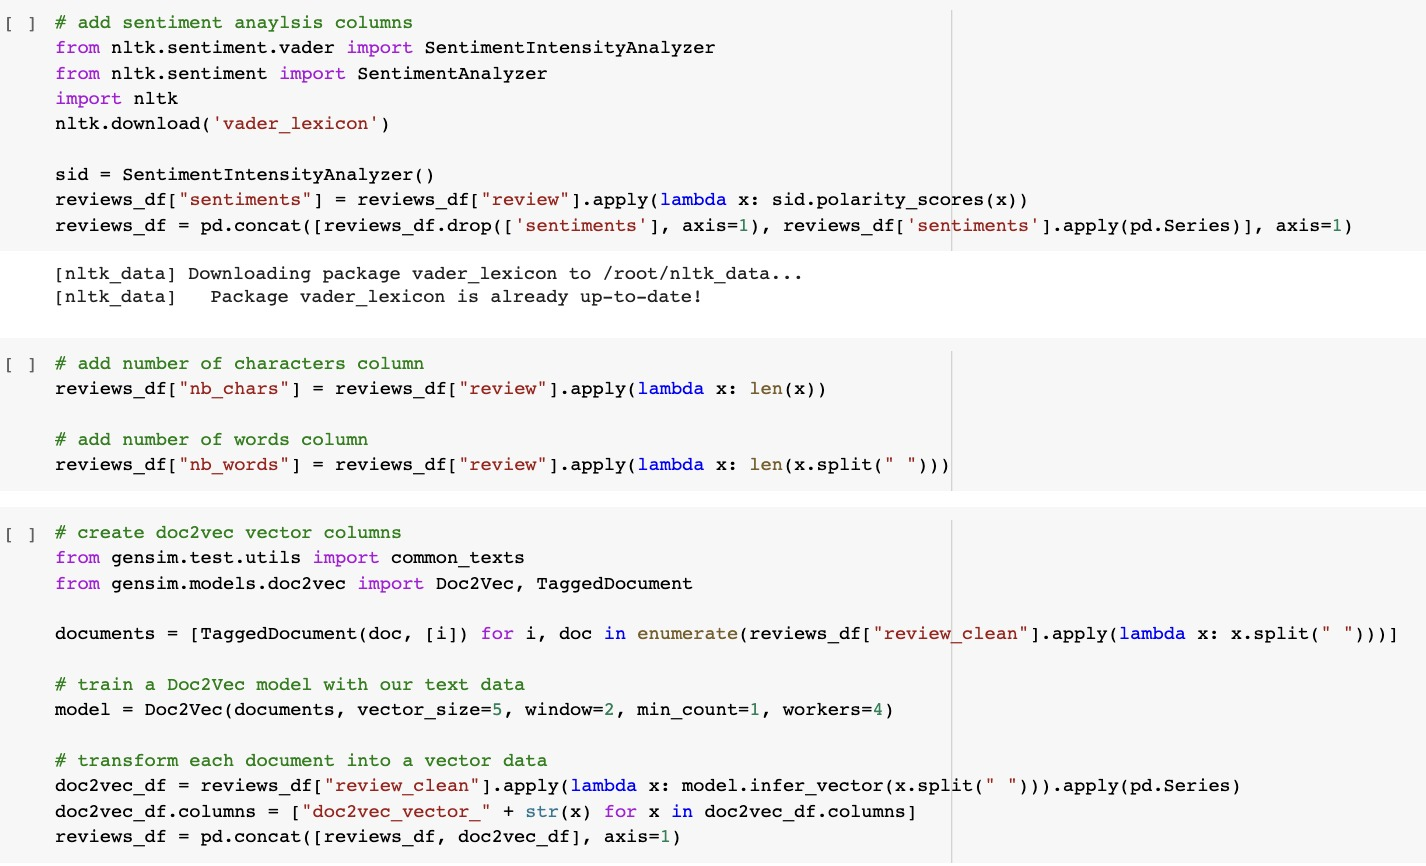
\includegraphics[width=9.5cm, height=12cm \textwidth]{sentiment analysis.jpeg}
Here, after finishing all the cleaning processes the next step is to assign polarity scores to the reviews in the dataset. Below is the code for SentimentIntensityAnalyzer.A sentiment intensity analyzer assigns a numerical value to the sentiment expressed to a text, typically on a scale from -1 to 1. It uses NLP and machine learning algorithms to recognize patterns and identify sentiment.Sentiment intensity analyzers can be used to monitor customer feedback and product reviews, providing insights into the sentiment of a large volume of text data to inform business decisions and improve customer satisfaction.\\

For example in below image we can see sentiment polarity scores for the review in the text is "The bar was shut when I got back at midnight which seemed quite early for a hotel bar on a Saturday night in a city like Amsterdam". \{'neg': 0.0, 'neu': 0.898, 'pos': 0.102, 'compound': 0.3612\}.

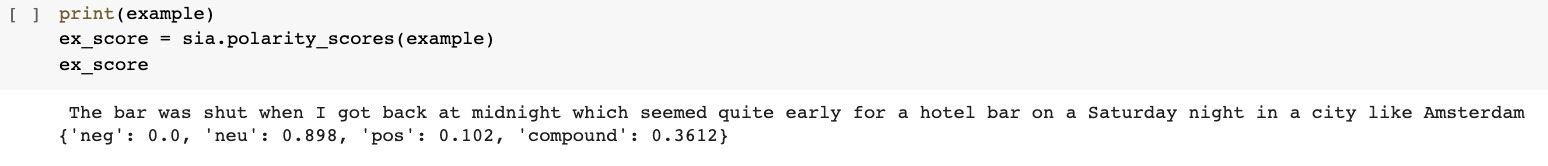
\includegraphics[width=9cm, height=2.75cm \textwidth]{sia pol.jpeg}

we can plot sentiment distribution curve using sentimental scores which we got, 1 reprsents good review and 0 as bad review.

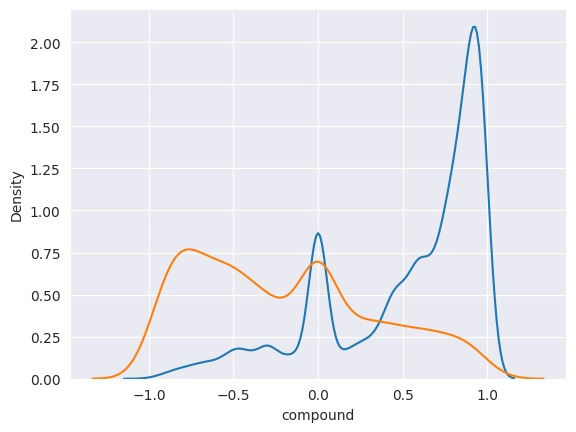
\includegraphics[width=9cm, height=6cm \textwidth]{density.jpeg}
\subsection{Data Classification}
In our method we have used two methods to classify the data they are  Random Forest Classifier and RoBERTa using Transformers.
\subsubsection{Random Forest Classifier}
It is s popular algorithm for classification and regression issues is the supervised machine learning technique known as random forest. It creates decision trees from several samples, using the majority vote for classification and the average for regression.
The "forest" it creates is an ensemble of decision trees, often trained using the "bagging" approach.\\

 Bagging: The final result is based on majority vote and a separate training subset is created using replacement from a sample of the training data. 

In Random Forest we have these advantages such as Diversity, Parallelization, Train-Test Split, and Stability are important features of a random forest, which reduces feature space, uses CPU, and is based on majority voting.\\

Steps involved in training our dataset are we have imported necessary libraries from Sklearn ensemble Random Forest classifier and model select to train split our dataset features selected.\\

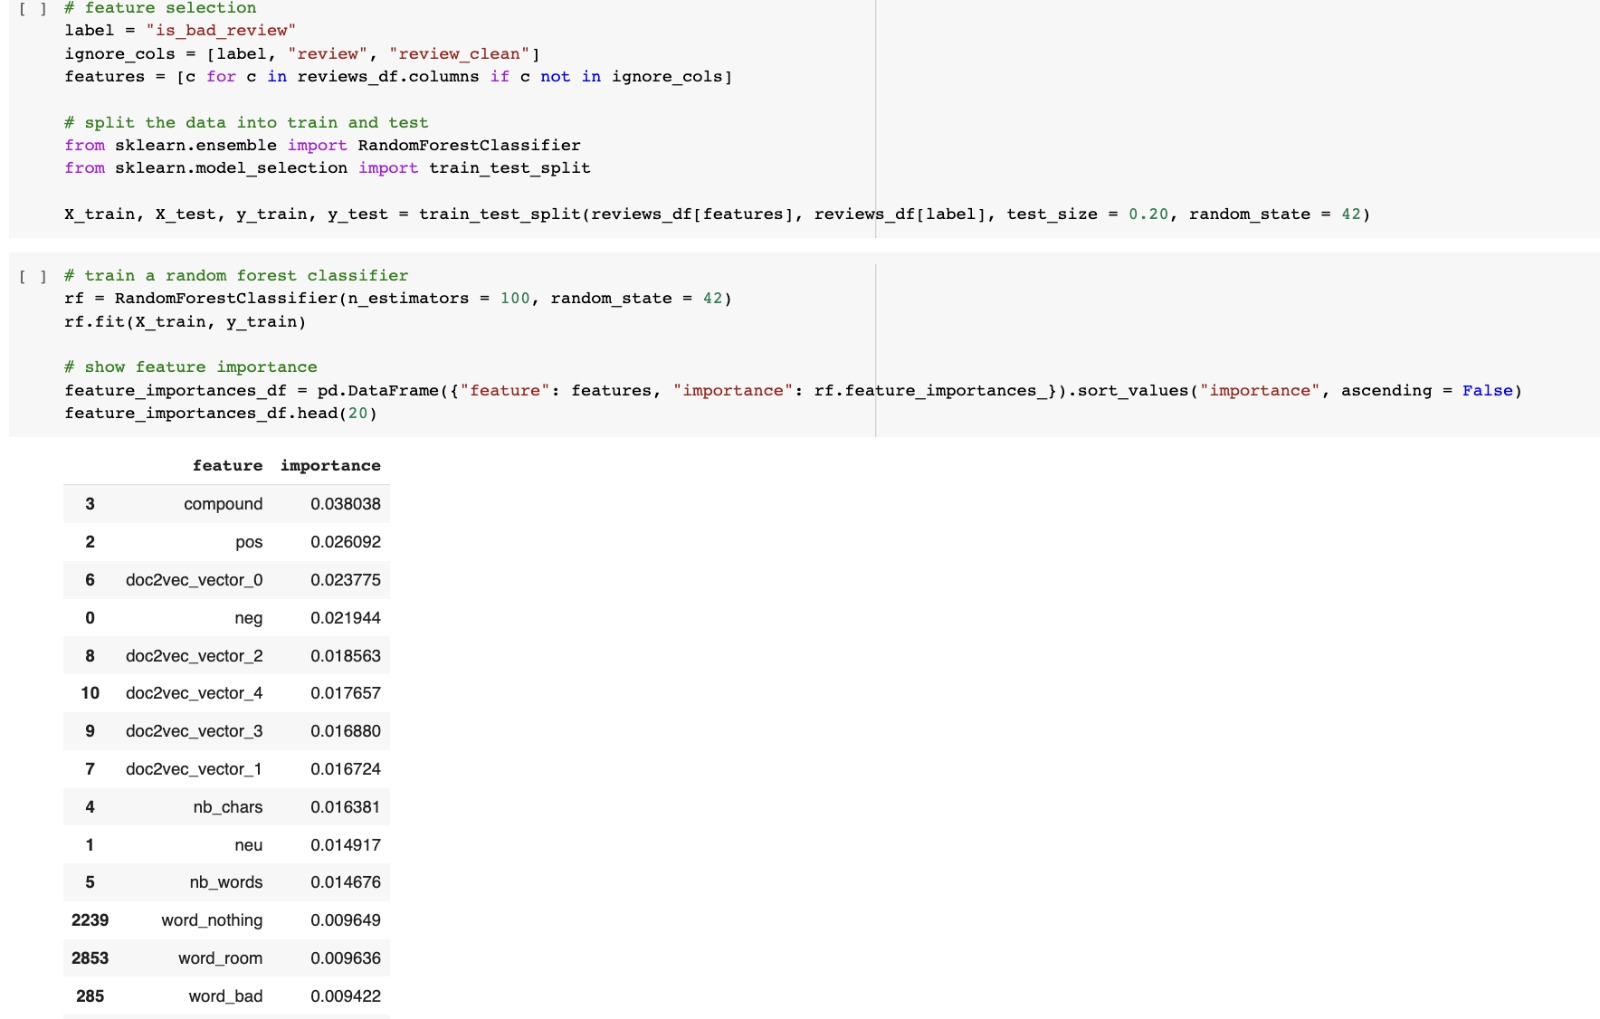
\includegraphics[width=9.5cm, height=8cm \textwidth]{rf.jpeg}\\

We have used hyperparameters like n\_estimators and random-state and trained the dataset with different set of values.

\subsubsection{RoBERTa using Transformers}
A variation of BERT that changes the pretraining procedure is called RoBERTa. The modifications includes for training models, longer, larger batch sizes. Training on longer sequences, deleting the next sentence prediction aim, adjusting the masking pattern dynamically applied to the training data.
By dynamically changing the masking pattern applied to the training data and removing the objective training for next sentence prediction on longer sequences.\\
Here, we have used pretrained cardiffnlp/twitter-robberta analysis for training our dataset.\\
Steps involved in roberta process are installing necessary libraries which are required for our model. They are AutoTokenizer, AutoModelForSequenceClassification, and softmax. Here we have taken a subset of 1000 reviews which are there in the dataset. Next step is to encode the text with tokenizer, using pretrained model we running the dataset and then applying the softmax in order to get polarity scores.
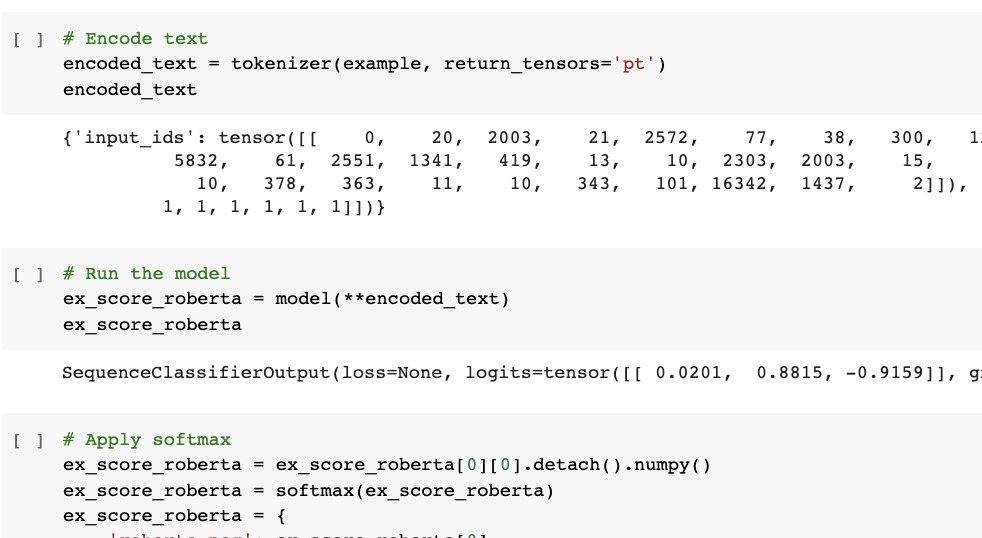
\includegraphics[width=9.5cm, height=8cm \textwidth]{encode.jpeg}\\

\subsection{Performance and Evaluation }
\subsubsection{Random Forest Model}
A receiver operating characteristic (ROC) curve shows how well a model can categorize binary outcomes. An ROC curve is created by displaying a model's false positive rate vs its true positive rate for each feasible cutoff value. The area under the curve (AUC) is frequently measured and used as a statistic to demonstrate how well a model can identify data points.\\

The ROC (Receiver Operating Characteristic) curve is frequently employed to summarize the quality of our classifier. The better predictions are, the higher the curve is above the diagonal baseline. \\
Although the AUC ROC (Area Under the Curve ROC) is excellent, we should not use it to evaluate the quality of our model here. Because our dataset is imbalanced, the  Negatives corresponds to our number of positive reviews, which is very high. \\
This means that even if there are some instances of false positives, our FPR will remain very low. Our model will be able to forecast many false positives while maintaining a low false positive rate, while raising the genuine positive rate and therefore artificially improving the accuracy.




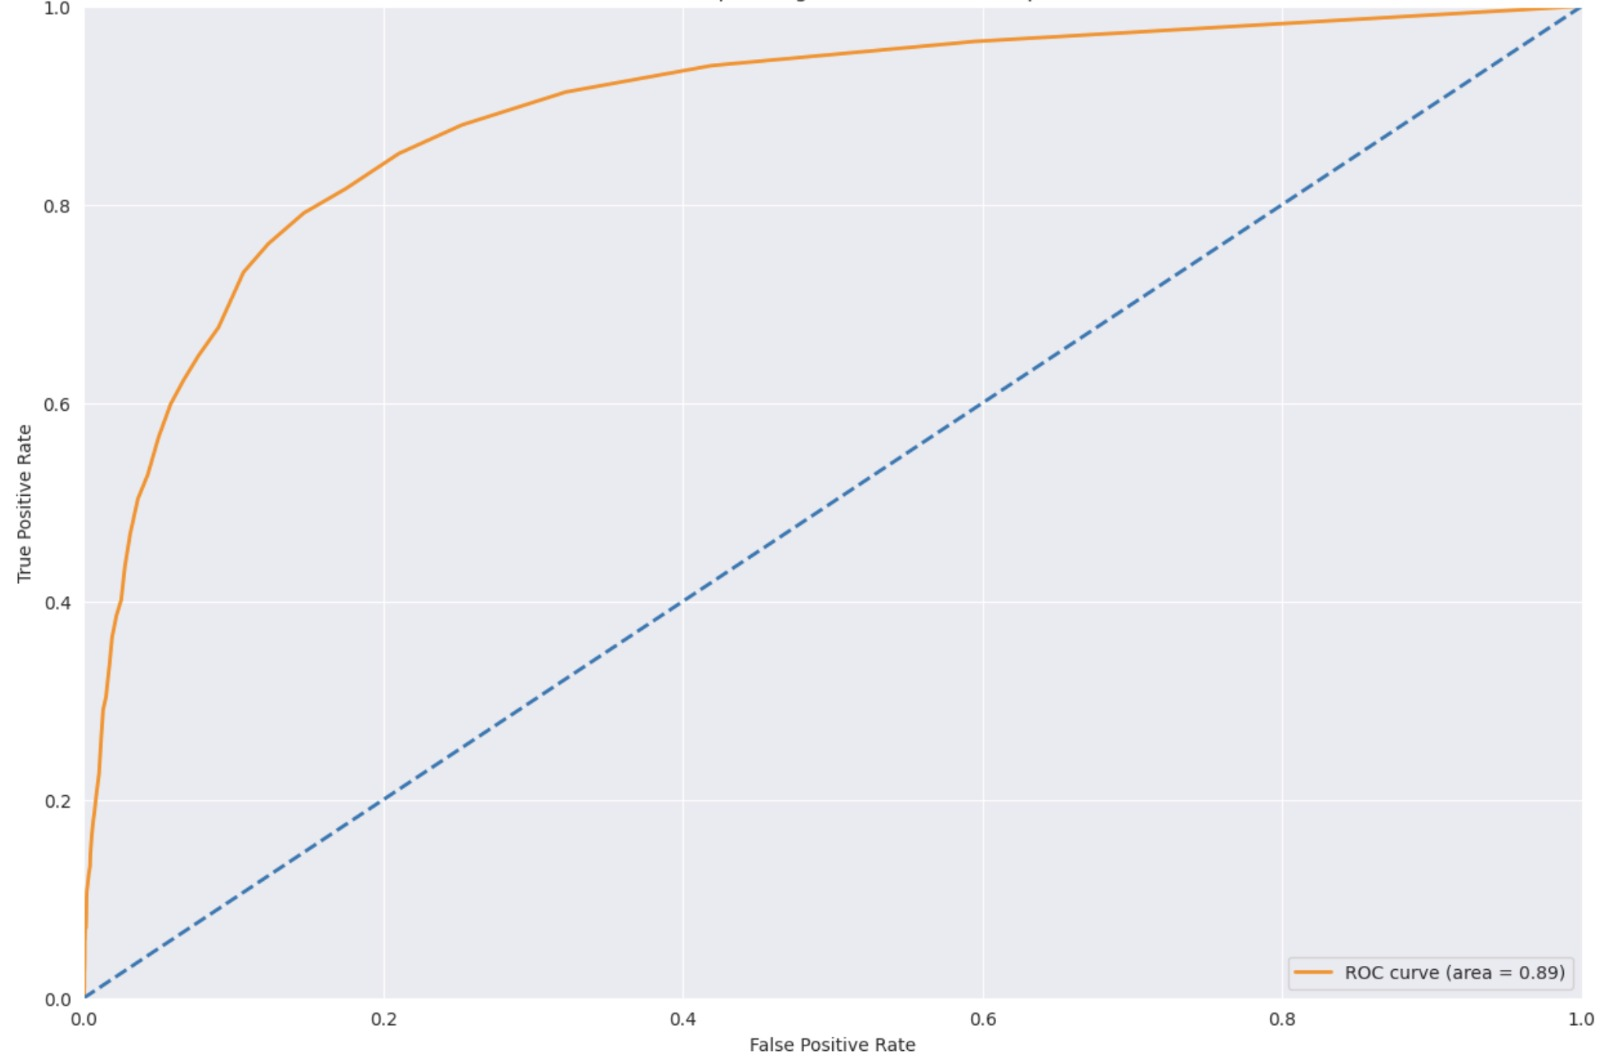
\includegraphics[width=9cm, height=6cm \textwidth]{roc.jpeg}\\

In order to calculate the PR Curve we have here precession and recall. Precision (also called positive predictive value) is defined as the number of true positives divided by the total number of positive predictions. Hence, precision quantifies what percentage of the positive predictions were correct: How correct our model's positive predictions.Recall (also called sensitivity) is defined as the number of true positives divided by the total number of true positives and false negatives (i.e. all actual positives). Hence, recall quantifies what percentage of the actual positives you were able to identify: How sensitive our model was in identifying positives.
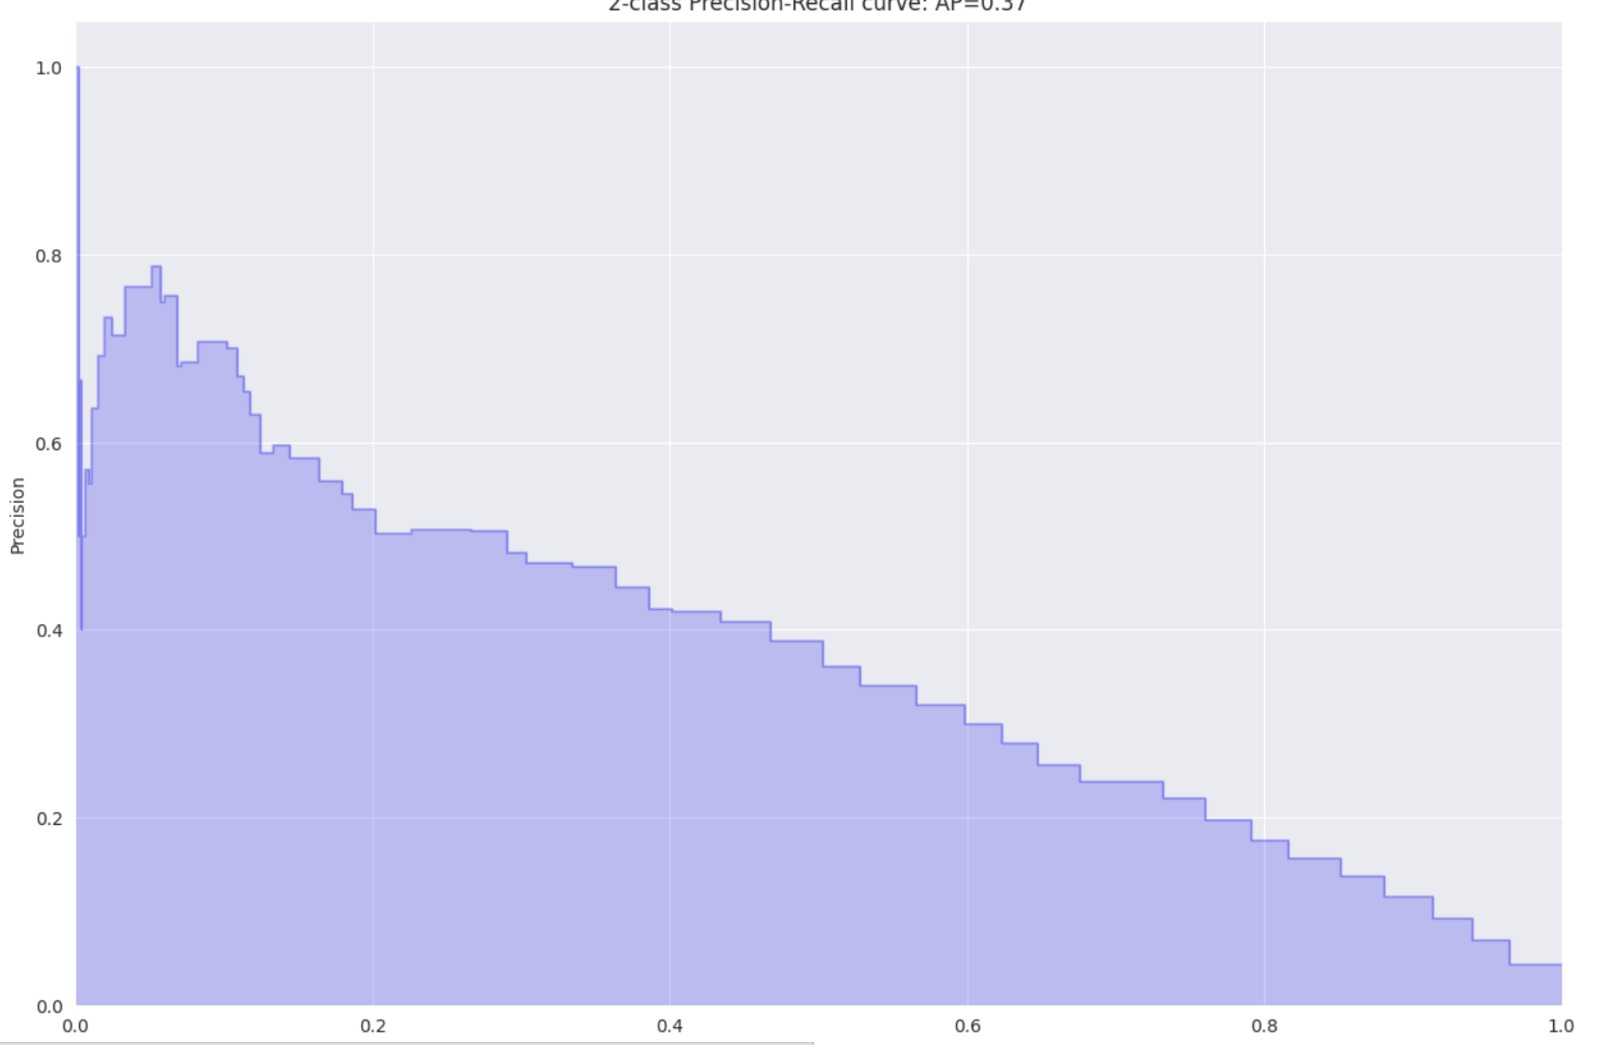
\includegraphics[width=9.5cm, height=8cm \textwidth]{pr.jpeg}\\

After experimenting with various N-Estimators and Random State values, the Random Forest Classifier achieved the highest accuracy of 0.89 for the ROC and 0.34 for the PR curves.\\

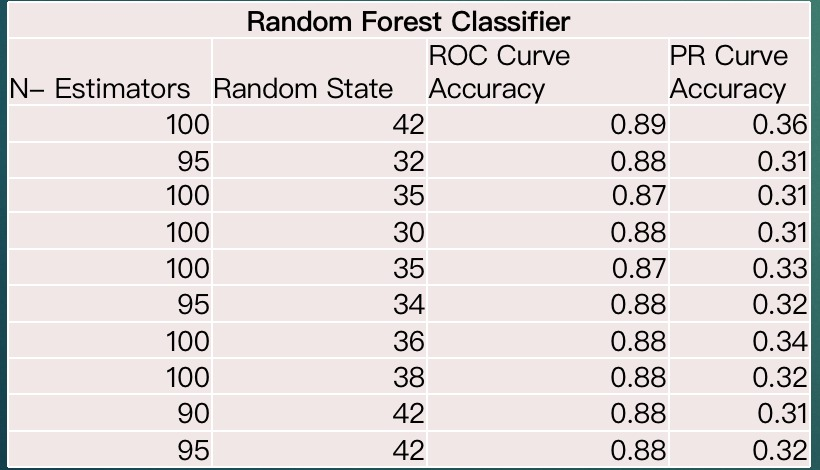
\includegraphics[width=9.5cm, height=8cm \textwidth]{ra.jpeg}\\
\subsubsection{Transformers Model}
Another strategy using Transformers yields an accuracy of 0.99 in Vader and 0.94 in Roberta.Here, at first we have taken subset of 1000 reviews and done sentimental analysis on all the dataframe subset taken from the dataset.

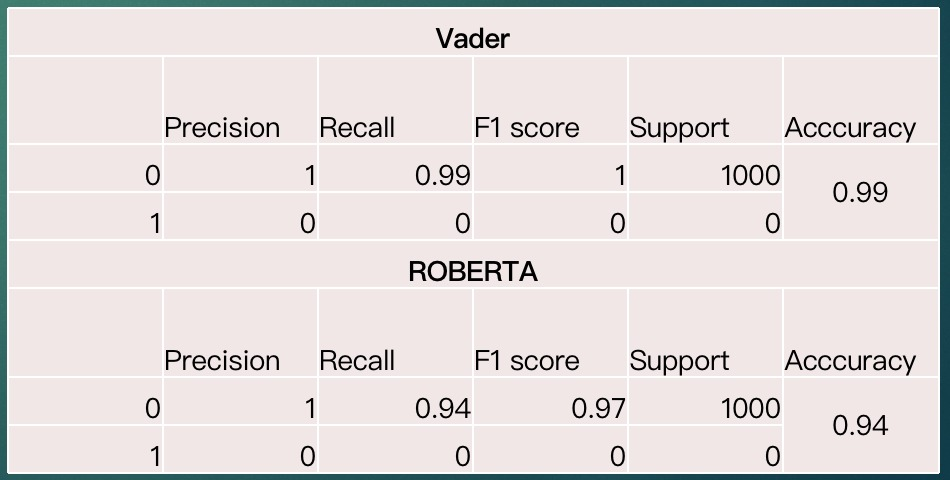
\includegraphics[width=9.5cm, height=9cm \textwidth]{vader and roberta.jpeg}\\
\section{Conclusion}
\begin{enumerate}
    \item Obtaining a ROC score of 0.89, which makes it very good and trust worthy in generating predictions on hotel reviews.
    \item We have a precision recall curve to back this up. The chart clearly shows that as recall increases, precision drops. This demonstrates the importance of selecting a prediction threshold that is appropriate for our needs.
    \item As a result, the Random Forest classifier performed admirably when generating final predictions.
    \item The Gensim module generates a vector of numbers that represents every word in the corpus based on the situations in which they appear (Word2Vec), which makes it quite intriguing.
    \item In general Roberta has high accuracy when compared to Vader but in our model as we have taken subset of reviews so we got vader higher accuracy.
    
    
\end{enumerate}

\section{References}
\begin{enumerate}



\item Sarah Anis, Sally Saad and Mostafa Aref [2020].
Sentiment Analysis of Hotel Reviews Using Machine Learning Techniques. Part of the Advances in Intelligent Systems and Computing book series (AISC,volume 1261).
\item Nandal, N., Tanwar, R. and Pruthi, J. Machine learning based aspect level sentiment analysis for Amazon products. Spat. Inf. Res. 28, 601–607 (2020).
\item Shaziya, Humera, G. Kavitha, and Raniah Zaheer. "Text categorization of movie reviews for sentiment analysis." International Journal of Innovative Research in Science, Engineering and Technology 4.11 (2015): 11255-11262.


\item Kamal, Ahmad. Review mining for feature based opinion summarization and visualization. arXiv preprint arXiv:1504.03068 (2015).


\item Appel, O., Chiclana, F., Carter, J., and Fujita, H. (2016). A hybrid approach to the sentiment analysis problem at the sentence level. Knowledge-Based Systems, 108, 110–124.
\item https://medium.com/analytics-vidhya/tf-idf-term-frequency-technique-easiest-explanation-for-text-classification-in-nlp-with-code-8ca3912e58c3
\item https://medium.com/swlh/bag-of-words-code-the-easiest-explanation-of-nlp-technique-using/
\end{enumerate}
%\subsection{Sub section 2}\label{Subsection2}

%You can add sub section 2 here. Or you can add more subsection under any section. I am cross 
%refferencing the sub section here ~\ref{Subsection1}. You just need to add a \textbf{label} on any section or subsection you want 
%refer at any point. Then you need to add a command similar to this \~\\ref{Subsection1}. 
%You can also bold any text with \\textbf\{\} and italic with \\textit\{\}  command. 
%Here is an 

%\subsection{Subsection with table}

%You can add table also. there are many nice latex table builder online. They will give you option to edit the data in the table manualy 
%And generate the latex code for you. Then you can copy the latex code here. Or you can build the table in power point and 
%export  it a s a figure. Then add the figure in the latex file.

%Following is a sample table with latex code. the command for adding figure is given at the later part of the file. 


%\begin{table}[h]
  %\centering{
 % \begin{tabular}{|l|l|}
 % \hline
  %Column 1 & Column 2 \\ \hline
  %data     & data     \\ \hline
  %data     & data     \\ \hline
 % \end{tabular}
 % }
%\end{table}





%========================================================================================================================
%\section{Background} \label{BackgroundSection} 
%========================================================================================================================


%Here is an example of how to add a figure. You can add any figure with this command. 




%\begin{figure}[h]
 %\centering
% \includegraphics[trim=0in 1in 0in 0, clip,scale=.345]{Pipeline.pdf}
 % \caption{\centering V1Model pipeline architecture}
% \caption{ V1Model pipeline architecture}
 %\label{fig:V1ModelArchitecture}
%\end{figure}












%========================================================================================================================
%\section{Conclusion}  \label{Conclusion}
%========================================================================================================================
%Write your conclusin here. There are some reference to my papers in the compiler.bib file. You can cite them in your report. You can
%also add citation for any other paper or report or website. The command for citing some work is 
%~\cite{robin2022clb}, ~\cite{robin2021p4kp}, ~\cite{robin2022p4te}, ~\cite{robin2022preprint}. But before adding citation you need to add the bibtex entry in the compiler.bib file. 


%========================================================================================================================
%\section{How to compile} 
%========================================================================================================================
%There is a Makefile in the folder. It lists the steps to compile the latex file and generate the pdf. Alternatively you can take the 
%compiler.tex and compiler.bib file and any other figure you want to use; then use the overleaf online editor. That is easier because it will not need
%installing latex in your own PC. Easy writing. 

%-------------------------------------------------------------------------------
% Don't change the follwoing two lines. They are for formatting the file. 
%\bibliographystyle{unsrt}
%\bibliography{Compiler}



%%%%%%%%%%%%%%%%%%%%%%%%%%%%%%%%%%%%%%%%%%%%%%%%%%%%%%%%%%%%%%%%%%%%%%%%%%%%%%%%

%\appendix
%\subsection{\textit{QoS-Modifer} P4 Program}\label{App:QoSModiferP4Program}
%==========================================================================
%This is an example if you want to write an algorithm or add source code. 

%\small{
%\begin{lstlisting}[linewidth=\columnwidth,breaklines=true,frame = single]

%}
%\end{lstlisting}
%}











\end{document}

%%%%%%%%%%%%%%%%%%%%%%%%%%%%%%%%%%%%%%%%%%%%%%%%%%%%%%%%%%%%%%%%%%%%%%%%%%%%%%%%

%%  LocalWords:  endnotes includegraphics fread ptr nobj noindent
%%  LocalWords:  pdflatex acks